%% jumplines_example.tex -- Example usage file
%%%
%% -------------------------------------------------------------------------------------------
%% Copyright (c) 2015 by Dr. Christian Hupfer <christian dot hupfer at yahoo dot de>
%% -------------------------------------------------------------------------------------------
%%
%% This work may be distributed and/or modified under the
%% conditions of the LaTeX Project Public License, either version 1.3
%% of this license or (at your option) any later version.
%% The latest version of this license is in
%%   http://www.latex-project.org/lppl.txt
%% and version 1.3 or later is part of all distributions of LaTeX
%% version 2005/12/01 or later.
%%
%% This work has the LPPL maintenance status `maintained'.
%%
%% This work consists of all files listed in README
%%


\documentclass[12pt,a4paper,twocolumn,languages=english]{article}


\usepackage{graphicx}%
\usepackage{blindtext}%
\usepackage[languages=spanish,ngerman]{jumplines}

\usepackage{hyperref}
\usepackage{bookmark}
\usepackage[babel,style=english]{csquotes}

\newcommand{\myquotes}[1]{\enquote{#1}}%

\begin{document}


\listofarticle
\listofcontarticle


\clearpage


\JumplineArticle[TeaserHeight=2.25in,ArticleHeadline={Breaking News}]{%
  \Large\textbf{Nothing special on the dark side of the moon}\par
  \begin{center}
\includegraphics[scale=0.3]{example-image-a}\end{center}\par
  \blindtext[2]
}
%
\JumplineArticle[RightHere=true,TeaserHeight=2in,ArticleAuthor={Gandalf},ContinuedOnTopskip=0.5cm,ContinuedOnBottomskip=10cm,TeaserHeaderContent={A short article}]{\color{red}{\blindtext[10]}}%
\JumplineArticle[TeaserHeight=2in,ContinuedArticleHeaderContent={More information},TeaserHeaderColor={yellow}]{\textcolor{blue}{\blindtext[1]\textcolor{Green}{Showing}\blindtext[2]}}%
\JumplineArticle[TeaserHeight=3in,ArticleHeadline={\Huge Breaking News}][Breaking News]{\Huge \sffamily The World is a Globe\par\begin{center}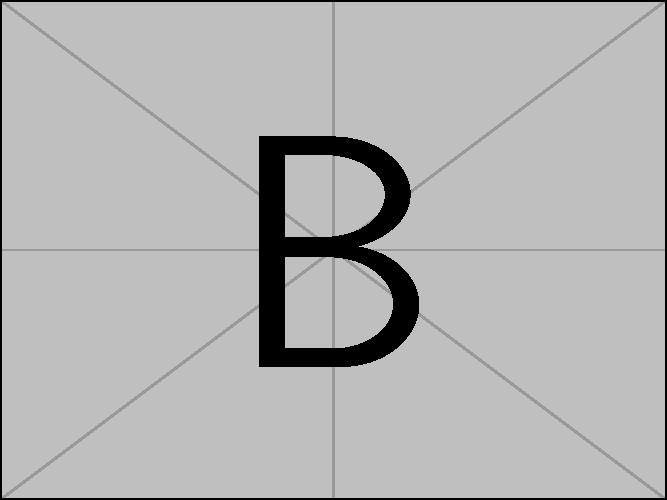
\includegraphics[scale=0.3]{example-image-b}\end{center}\par
  {\color{violet}{\( E = mc^2\)}}}%
\selectlanguage{spanish}
\JumplineArticle[TeaserHeight=2in][My Headline]{\color{brown}{\blindtext[10]}}%
\JumplineArticle[TeaserHeight=8in,emptyarticleinbookmarks=true]{\textcolor{blue}{\blindtext[10]}}%
\JumplineArticle[TeaserHeight=2in,ArticleHeadline={A golden rod text},BookmarkEntry={\textcolor{GoldenRod}{Golden rod}}]{\textcolor{Goldenrod}{\blindtext[10]}}%
\JumplineArticle[TeaserHeight=2in,emptyarticleintoc=true,emptyarticleinbookmarks=true,autobookmark=false,ArticleAuthor={\textcolor{violet}{Some guy from the LaTeX3 - team}}]{\Huge \begin{center}
\includegraphics[scale=0.2]{example-image-c}\end{center} \centering ``I can't wait for \LaTeX3 -- it's so exciting''}




\clearpage


\ShipoutArticleTeasers%
\clearpage

\ShipoutArticleHangingArticles%

\end{document}